\chapter{Flujo multiagente del sistema}

\section{Funcion de este capitulo}

Este capitulo es uno de los nucleos del nuevo TFM. Aqui no basta con decir que el sistema usa varios agentes: hace falta explicar con detalle como circula la informacion, que hace cada bloque, que controles existen y por que esa organizacion mejora la trazabilidad y la explicabilidad del analisis.

La idea central que conviene sostener en todo el capitulo es la siguiente: el valor del sistema no esta solo en producir una respuesta final, sino en hacerlo mediante un flujo auditable, con artefactos observables y con decisiones tecnicas que permitan entender que ha ocurrido en cada etapa.

\section{Preguntas que debe responder el capitulo}

\begin{enumerate}
    \item ?Que recibe exactamente el sistema y como se transforma esa entrada a lo largo del flujo?
    \item ?Que hace cada bloque principal y por que ese bloque es necesario?
    \item ?Que diferencia hay entre el flujo principal y los mecanismos de correccion?
    \item ?Que papel tienen los prompts como contrato operativo de los agentes?
    \item ?Que evidencias deja el sistema para poder reconstruir una ejecucion completa?
    \item ?Por que este flujo es mas explicable y controlable que una respuesta directa del LLM?
    \item ?Que decisiones de diseno ayudan a justificar luego la metodologia y la evaluacion?
\end{enumerate}

\section{Vision general del flujo}

La Figura~\ref{fig:flujo_multiagente_final} se toma como referencia de alto nivel para el desarrollo del nuevo TFM. En ella se representa el recorrido completo desde la solicitud inicial del usuario hasta la respuesta final, incluyendo los agentes principales, los subagentes de correccion y los puntos de validacion mas relevantes.

\begin{figure}[htbp]
\centering
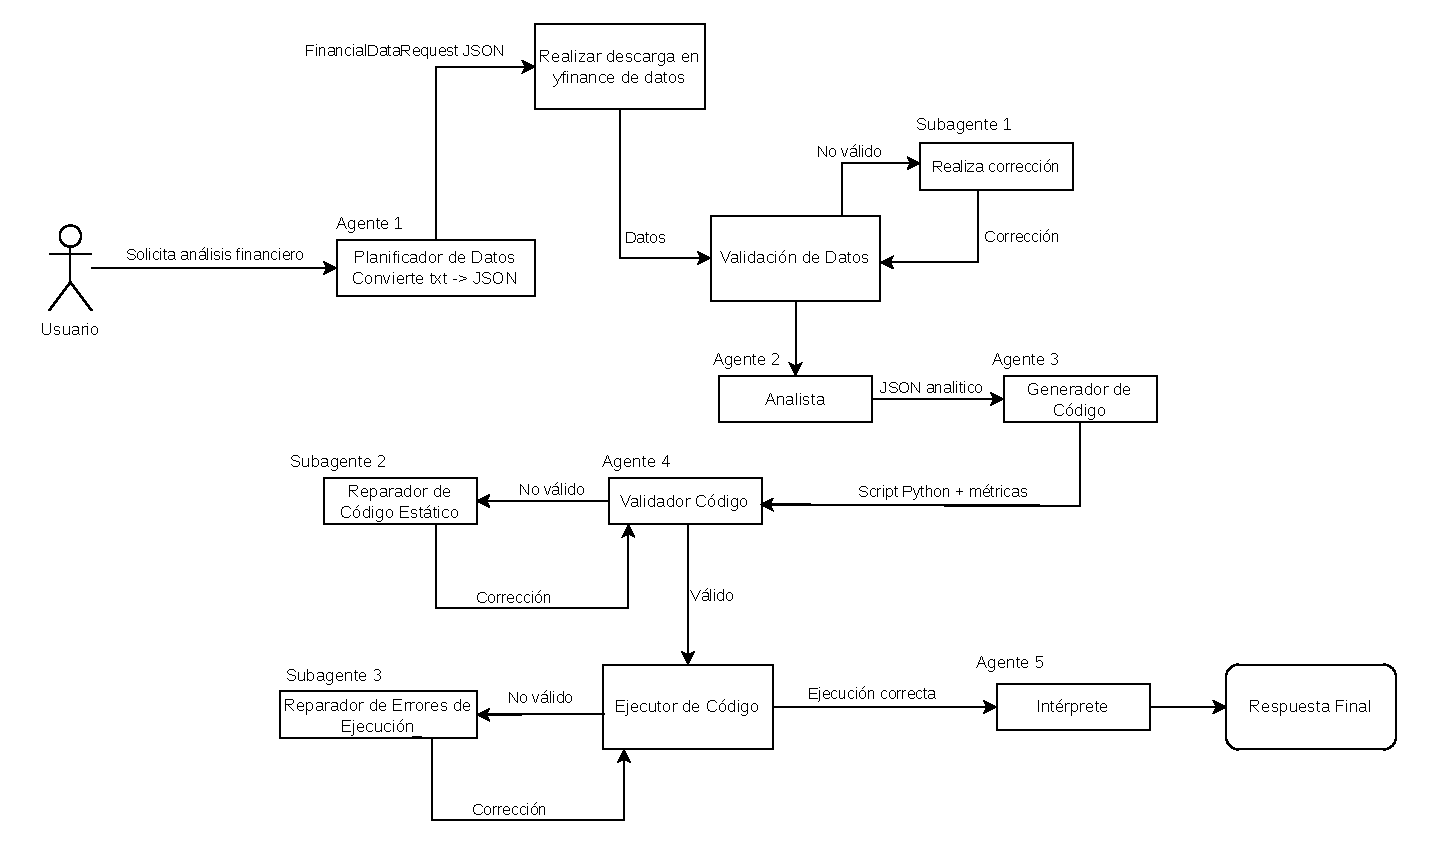
\includegraphics[page=1,width=\textwidth]{../FlujoFinal.drawio.pdf}
\caption{Flujo multiagente de referencia para el desarrollo del sistema de analisis financiero.}
\label{fig:flujo_multiagente_final}
\end{figure}

\textit{Completar aqui una lectura global de la figura. Conviene describir el recorrido principal sin entrar todavia en todos los detalles tecnicos: que entra en el sistema, como se prepara la informacion, donde intervienen los agentes, en que puntos se valida el proceso y como se llega a la respuesta final. Este primer apartado debe servir para que el lector no se pierda cuando empiece el detalle del flujo.}

\textit{Tambien conviene adelantar aqui dos ideas que luego se desarrollaran mejor: que la arquitectura busca separar responsabilidades y que esa separacion hace posible explicar mejor el comportamiento del sistema, detectar fallos y conservar evidencias del proceso.}

\section{Entrada y estado compartido}

\subsection{Entrada del sistema}

\textit{Completar aqui que estructura recibe el sistema, que campos son obligatorios y que informacion no debe inferirse de forma libre. Conviene explicar si la entrada incluye consulta, tickers, rango temporal, rutas de CSV, avisos y cualquier otro campo relevante. Tambien es importante dejar claro que el sistema no recibe una etiqueta previa de complejidad o profundidad de respuesta: los agentes deben inferirla a partir de la propia consulta y de sus requisitos.}

\textit{En este apartado deberias poder explicar con comodidad por que la calidad de la entrada condiciona el resto del flujo y que errores se quieren evitar ya desde el primer momento.}

\subsection{Estado compartido}

\textit{Completar aqui que informacion se va guardando durante la ejecucion y por que existe un estado compartido. Lo importante no es solo enumerar campos, sino justificar para que sirve cada grupo de informacion: entrada normalizada, plan analitico, codigo generado, resultados de ejecucion, respuesta final, errores y avisos.}

\textit{Este apartado debe ayudarte a defender la trazabilidad del sistema. El lector tiene que entender que la respuesta final no aparece de forma opaca, sino que puede reconstruirse a partir de un historial estructurado de artefactos y transiciones.}

\section{Flujo principal del sistema}

\textit{Este bloque debe contar el recorrido principal del sistema de forma limpia, sin detenerse todavia en todos los bucles de correccion. La idea es explicar que hace cada fase, que recibe, que produce y por que es necesaria dentro del flujo completo.}

\subsection{Parte de datos}

\textit{Completar aqui todo el tramo inicial del flujo, desde la recepcion de la consulta hasta dejar preparada la informacion necesaria antes de entrar en el analisis principal. Puedes comentar normalizacion de la entrada, comprobacion de campos, seleccion o verificacion de CSV, coherencia entre consulta y datos disponibles y cualquier validacion temprana que reduzca errores posteriores.}

\textit{Aqui conviene insistir en que esta fase no intenta resolver la consulta, sino preparar el contexto de trabajo con la mayor claridad posible. Desde el punto de vista de la explicabilidad, este bloque debe mostrar que el sistema no empieza a generar codigo sin haber delimitado antes con que datos puede trabajar y bajo que restricciones.}

\subsection{Analista y generador de codigo}

\textit{Completar aqui como se transforma la peticion del usuario en un plan analitico y despues en un procedimiento ejecutable. Tiene sentido explicar juntos estos dos pasos porque forman un mismo bloque conceptual: traducir una intencion expresada en lenguaje natural a una secuencia de calculos concreta.}

\textit{En esta parte deberias comentar, al menos, que decide el agente analista, que restricciones recibe el generador de codigo, como se conecta el plan con el script final y que riesgos aparecen en esta traduccion. Tambien es un buen sitio para subrayar que el sistema no pide al LLM una conclusion financiera directa, sino un plan y un codigo trazable que luego sera sometido a controles.}

\subsection{Validacion del codigo}

\textit{Completar aqui como se revisa el codigo antes de ejecutarlo. Interesa explicar que se comprueba, por que se comprueba y que tipo de errores o conductas se quieren bloquear: uso de operaciones no permitidas, incumplimiento del contrato de entrada o salida, accesos inseguros, estructura incorrecta o ausencia de controles minimos.}

\textit{Este bloque es muy importante para defender el diseno del sistema. Desde el punto de vista de la memoria, aqui puedes explicar por que generar codigo no es suficiente y por que la validacion previa es una condicion necesaria para poder hablar de un flujo controlado.}

\subsection{Validacion de ejecucion}

\textit{Completar aqui que ocurre una vez que el codigo ya se lanza: control del proceso, recogida de \texttt{stdout} y \texttt{stderr}, interpretacion del codigo de retorno, comprobacion de que la salida tenga el formato esperado y deteccion de fallos de calculo o inconsistencias.}

\textit{Conviene dejar claro que ejecutar no equivale automaticamente a obtener un resultado valido. Esta fase debe mostrar que el sistema tambien controla lo que ocurre despues de la generacion de codigo y que la ejecucion se evalua como una evidencia tecnica, no solo como un paso ciego.}

\subsection{Interpretacion y respuesta final}

\textit{Completar aqui como se transforma la salida estructurada en una respuesta final en espanol. Lo importante es explicar que esta etapa no recalcula ni inventa resultados, sino que interpreta lo ya obtenido y lo comunica de forma clara, prudente y ajustada a la consulta del usuario.}

\textit{Este apartado es un buen lugar para destacar la explicabilidad externa del sistema: no solo interesa que el flujo sea auditable por dentro, sino que la respuesta final tambien sea comprensible para un lector humano y deje claros los resultados observados, su lectura y sus limitaciones.}

\section{Subagentes de correccion y recuperacion}

\textit{Completar aqui el papel de los subagentes o mecanismos de reparacion. Conviene separarlos del flujo principal para que primero se entienda el recorrido base y despues se vea como reacciona el sistema cuando algo falla.}

\textit{En este apartado deberias poder explicar cuando se activa cada correccion, que informacion recibe el subagente, que tipo de error intenta reparar y que criterio decide si el flujo continua o termina en error. Tambien interesa comentar si las reparaciones afectan al plan, al codigo, a la ejecucion o solo a una parte concreta del proceso.}

\textit{Metodologicamente, esta seccion es importante porque muestra que el sistema no solo tiene una ruta ideal, sino tambien una estrategia controlada para gestionar fallos.}

\section{Diseno de prompts y contratos de los agentes}

\textit{Este es el lugar adecuado para incluir los prompts dentro de la memoria principal. No conviene tratarlos como un anexo aislado, sino como parte del diseno operativo del sistema.}

\textit{Completar aqui que objetivo tiene cada prompt, que entrada recibe cada agente, que salida se le exige y que restricciones guian su comportamiento. Puedes apoyarte en una tabla resumen y despues desarrollar los agentes mas importantes de forma narrativa.}

\begin{table}[htbp]
\centering
\small
\begin{tabularx}{\textwidth}{L{0.17\textwidth}L{0.20\textwidth}L{0.20\textwidth}Y}
\toprule
\textbf{Agente} & \textbf{Entrada principal} & \textbf{Salida esperada} & \textbf{Aspectos del prompt que conviene explicar} \\
\midrule
Agente de analisis & \textit{Completar} & \textit{Completar} & \textit{Objetivo, metricas, restricciones, estructura del plan.} \\
Agente de codigo & \textit{Completar} & \textit{Completar} & \textit{Contrato tecnico, imports permitidos, formato de salida, limites de seguridad.} \\
Agente de interpretacion & \textit{Completar} & \textit{Completar} & \textit{Uso exclusivo de resultados ejecutados, tono, prudencia y estructura de respuesta.} \\
Subagentes de correccion & \textit{Completar} & \textit{Completar} & \textit{Tipo de error que reciben, alcance de la reparacion y limites de actuacion.} \\
\bottomrule
\end{tabularx}
\caption{Guia para documentar los prompts y contratos de los agentes.}
\label{tab:prompts_contratos_agentes}
\end{table}

\textit{En este bloque debes poder defender no solo que existen prompts distintos, sino por que estan separados y que gana el sistema con esa especializacion. Si incluyes fragmentos textuales, conviene que sean los que mejor revelan el contrato de cada agente y no necesariamente el prompt completo sin explicacion.}

\section{Trazabilidad y artefactos generados}

\textit{Completar aqui que evidencias deja el sistema en cada ejecucion. Este apartado es clave para justificar que el flujo es auditable y explicable. Lo importante no es enumerar solo ficheros, sino explicar que papel cumple cada artefacto dentro de la reconstruccion del proceso.}

\textit{Puedes comentar, por ejemplo, la entrada normalizada, el plan analitico, el codigo generado, los logs de ejecucion, la salida estructurada, los avisos, los errores y la respuesta final. Conviene explicar que gracias a estos artefactos es posible revisar por que una respuesta fue correcta, insuficiente o fallida, y en que punto del flujo se produjo el problema.}

\textit{Este apartado conecta de forma natural con la metodologia y con la evaluacion posterior, porque deja claro que los resultados del TFM pueden defenderse con evidencias observables y no solo con impresiones subjetivas.}

\section{Decisiones de diseno}

\textit{Completar aqui por que se elige este flujo y no otro. Este apartado debe servir para justificar las principales elecciones de arquitectura: separacion de responsabilidades, uso de varios agentes, validacion previa a la ejecucion, reparacion controlada, anclaje a datos locales y conservacion de artefactos.}

\textit{No se trata de repetir la metodologia, sino de defender las decisiones tecnicas que hacen posible luego una evaluacion seria del sistema. En otras palabras, aqui explicas por que la arquitectura esta pensada para producir un analisis mas controlable, mas explicable y mas revisable que una respuesta directa generada de una sola vez por el modelo.}
